\chapter{p3 = 16 (1 graphs)}
\newpage\begin{figure}
  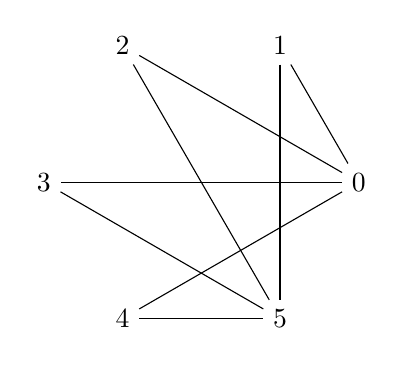
\begin{tikzpicture}
      \draw
        (0.0:2) node (0){0}
        (60.0:2) node (1){1}
        (120.0:2) node (2){2}
        (180.0:2) node (3){3}
        (240.0:2) node (4){4}
        (300.0:2) node (5){5};
      \begin{scope}[-]
        \draw (0) to (1);
        \draw (0) to (2);
        \draw (0) to (3);
        \draw (0) to (4);
        \draw (1) to (5);
        \draw (2) to (5);
        \draw (3) to (5);
        \draw (4) to (5);
      \end{scope}
    \end{tikzpicture}
\end{figure}
\begin{itemize}
\item signature: 111100001001011
\item g: Graph with 6 nodes and 8 edges
\item order: 6
\item size: 8
\item max degree: 4
\item degrees: 2,2,2,2,4,4
\item is tree: 0
\item is bipartite: 1
\item has bridge: 0
\item is chordal: 0
\item is complete: 0
\item min cycle basis weight: 12
\item min cycle basis size: 3
\item diameter: 2
\item radius: 2
\item is eulerian: 1
\item is planar: 1
\item number of faces: 4
\item is regular: 0
\item p3: 16
\item p4: None
\item property hash: e270bf8a5267498488e82c9573ba55a861a0ce330bfb3de8686eeb8b74e9a431
\end{itemize}
\newpage
